
% WARNINGS: 
%	    1. You must make sure that PDF output generated from this
%	       template is complete both when displayed with a viewer 
%	       (acroread, for example) and when printed on paper.
%	       LaTeX installations vary greatly and therefore it might 
%	       not be possible to get all proposals to come out 
%	       correctly with a single text page layout. 
%	       In some cases you will have to adjust the 
%	       \topmargin=-7mm command in the template to center the 
%	       text vertically in the page.  


\documentclass[12pt,a4paper]{article} 
\usepackage{times}
\usepackage{graphics,graphicx}
\usepackage[update,prepend]{epstopdf}
\usepackage[innercaption]{sidecap}
\usepackage{subcaption}
\usepackage{amssymb, amsmath}	       
\usepackage{xspace}				
\usepackage{natbibspacing, natbib}
\usepackage{aas_macros}
\usepackage{wrapfig}
\usepackage{floatrow}

\newcommand{\ncrit}{\mbox{$n_{\rm crit}$}\xspace}
\newcommand{\comol}{$^{12}$CO\xspace}
\newcommand{\Lsun}{\mbox{L$_{\odot}$}\xspace}
\newcommand{\LIR}{\mbox{$L_{\rm IR}$}\xspace}
\newcommand{\LFIR}{\mbox{$L_{\rm FIR}$}\xspace}
\newcommand{\rarr}{$\rightarrow$}
\newcommand{\aco}{\mbox{CO($J$=1\rarr0)}\xspace}
\newcommand{\bco}{\mbox{CO($J$=2\rarr1)}\xspace}
\newcommand{\cco}{\mbox{CO($J$=3\rarr2)}\xspace}
\newcommand{\eco}{\mbox{CO($J$=5\rarr4)}\xspace}
\newcommand{\rot}[3][HCN]{\mbox{#1($J$=#2\rarr#3)}\xspace} 
% default HCN; usage \rot[HCN]{3}{2} or \rot[\hcop]{4}{3}
\newcommand{\ahcn}{HCN($J$=1\rarr0)\xspace}
\newcommand{\dhcn}{HCN($J$=4\rarr3)\xspace}
\newcommand{\hcop}{HCO$^+$\xspace}
\newcommand{\ahcop}{\mbox{HCO$^+$($J$=1\rarr0)}}
\newcommand{\dhcop}{HCO$^+$($J$=4\rarr3)\xspace}
\newcommand{\Lp}[1][CO]{\mbox{$L^{\prime}_\textrm{\fontsize{8pt}{12pt}\selectfont{#1}}$}}
\newcommand{\LpU}{\mbox{K\,\,km\,\,s$^{-1}$\,\,pc$^2$}}
\newcommand{\kms}{km\,s$^{-1}$\xspace}
\newcommand{\pmOne}{\mbox{$^{-1}$}\xspace}
\newcommand{\Fig}[1]{Fig.~\ref{fig:#1}}
\newcommand{\Eq}[1]{Equation~\ref{eq:#1}}

%Compact BIB%%%%%%%%%%%%%%%%%%%%
\citestyle{aa}	
\bibliographystyle{apj_w_etal_3auth}

\usepackage{paralist}

\renewenvironment{thebibliography}[1]{%
%\section*{\refname}%
%  {\normalsize {\textbf{References:}}}
  \let\par\relax\let\newblock\relax%
  \inparaitem[{[}1{]}]}{\endinparaitem}
%%%%%%%%%%%%%%%%%%%%%%%%%%%%%


%%%%%%%%%%%%%%%%%%%%%%%%%%%%
%%%%%% Page dimensions %%%%%
%%%%%%	DO NOT CHANGE  %%%%%
%%%%%%%%%%%%%%%%%%%%%%%%%%%%

\textheight=247mm
\textwidth=180mm
\topmargin=-7mm
\oddsidemargin=-10mm
\evensidemargin=-10mm
\parindent 10pt

\renewcommand\floatpagefraction{.9}
\renewcommand\topfraction{.9}
\renewcommand\bottomfraction{.9}
\renewcommand\textfraction{.1}
% between fig
\setlength{\textfloatsep}{10pt plus 1.0pt minus2.0pt}
\setlength{\floatsep}{10pt plus 1.0pt minus 2.0pt}
\setlength{\intextsep}{10pt plus 1.0pt minus 2.0pt}
\setlength{\parskip}{0.01em}
\usepackage[small,tiny,compact]{titlesec}

\begin{document}
\pagestyle{plain}
\pagenumbering{arabic}
 
\begin{center}
{\large{\bf
{ 
Molecular gas dynamics and AGN/starburst mechanism in a
strongly-lensed wet merger: bridging the gap between local ULIRGs and high-z systems}
}}
\end{center}
\vspace{-0.545em}
\centerline{\normalsize{\bf PI: 
{T. K. Daisy Leung}}} 
%%%%%%%%%%%%%%%%%%%%%%%%%%%%%%%%%%
% \section*{Missing link between mergers/ULIRGs and their high-z analogues} 
% \vspace{-0.25em}
% \indent 
\vspace{0.1em} {\bf Missing link between mergers/ULIRGs and their high-z analogues} 
Ultraluminous infrared galaxies (ULIRGs: \LIR$\geq$10$^{12}$\Lsun) have been
regarded as analogues of high-redshift (z) starbursts given their
similarities in \LIR/\Lp\ and other physical properties.
% (e.g. high-z SB display morphological evidence of past or ongoing merger)
As such, detailed studies and characterization of ULIRGs are important 
to gain more detailed insight into the early universe and in studies of galaxy evolution over cosmic time.
It is believed that mergers play an important role in giving rise to these dusty galaxies
(e.g. Sanders \& Mirabel 1996). Yet, merger-induced effects on the physical mechanisms and chemistry 
that drive the intense starburst (SB) and active galactic nucleus (AGN) activities on small scales are still unclear.
Thus characterizing the properties of the molecular gas that fuels star-formation (SF) and AGN is
crucial to understand the interplay between AGN and SB
and their relation to the interstellar medium (ISM) properties of galaxies across cosmic time.

While the ISM in local ULIRGs has been studied in great detail with ALMA,
forming a rich inventory of molecular transitions that serves as the template for 
understanding high-z galaxies and galaxy evolution \citep[e.g.][]{Rangwala15a}, a wide knowledge gap persists
between $z$=0 and the epoch when most stars are formed in the universe ($z$$\sim$2). 
Understanding galaxy populations at the epoch when the build-up of stellar mass across cosmic
time is steeply rising is thus critical and we here aim to bridge this gap by testifying
correlations and properties found locally out to high/moderate redshifts by observing the 
dynamical structure of the different molecular gas components
in the quadruply lensed galaxy RXJ1131-1231 and its dust-obscured 
companion at $z_{\rm CO}$$\sim$0.65.
%to bridge the gap between nearby ULIRGs and their high-z analogues.

% \section*{Various molecular gas phases and the star-formation law} 
% \vspace{-0.25em}
\noindent {\bf Molecular gas in AGN/SB} 
Owing to the high molecular gas fractions in ULIRGs and their high-z analogues,
their extreme SFRs are a natural consequence of either gas is being converted into stars
more efficiently and/or their molecular gas content. Fragmentation
of giant star-forming clumps and turbulent conditions are also expected 
from gravitational instability of these gas-rich bodies. 
In fact, studies of the ISM kinematics at $z$=1-2 find clumps of size scale
 $\sim$few kpc \citep{Swinbank12a, Swinbank12b}. 
Resolving the gas dynamics on hundred pc scales is therefore an important first step
to understanding the mechanisms and physical processes taking
place on different scales and how the physical conditions 
are related to the starburst in ULIRGs at this epoch (when the SFR density is steeply rising).

While \comol emission traces the total molecular distribution and dynamics,
high-dipole moment molecules such as HCN and \hcop are expected to trace the 
properties of the denser, actively star-forming gas. Indeed, a tight correlation between \ahcn and \LIR 
(proxy for SFR) has been found in nearby galaxies and local giant molecular 
clouds (GMC; \citealt[hereafter GS04]{Gao04a}; \citealt{Wu05}), 
suggesting HCN is a faithful tracer of the star-forming dense gas.
% and that the origin can be attributed to the fundamental units of star formation. 
This has been supported by the linear correlations in 
\LIR-\Lp[\dhcn] and \LIR-\Lp[\dhcop] found recently \citep[hereafter Z14; see \Fig{SF}]{Zhang14a}, which also highlight 
the great utility of these mid-$J$ lines observable for galaxies at $z$$>$0.06.

Due to the difference in abundances and excitation conditions of HCN and \hcop
in star-forming versus AGN regions, the line ratio \ahcn/HCO$^+$($J$=1\rarr0) has been 
proposed as a diagnostic tool to separate emission originating from AGN and starburst
\citep{Kohno05a, Imanishi10, Izumi13a}. 
 %(e.g. HCO+ is enhanced in SF regions in PDRs and SN shocks and HCN is enhanced in AGN)
With the frequency coverage of ALMA, some studies have 
extended this diagnostic to using the J=4\rarr3 transitions 
\citep{Imanishi14a, GB14a, Viti14a}, where 
an elevated \dhcn/\dhcop line ratio is also seen in AGNs, suggesting
it, too, can be used to reveal a deeply buried AGN at the cores of ULIRGs \citep{Izumi16a, Imanishi16a}.

Prior to ALMA, studies of dense gas were largely limited to the local universe ($z\lesssim$0.1) 
with only five IR-luminous lensed galaxies detected at $z\gtrsim0.3$ 
(e.g. \citealt{Riechers06a, Riechers07a, Riechers10a, Wagg05a, Gao07a}).
However, none of these high-z detections spatially resolve the emission, rendering it difficult 
to draw conclusions on the dense gas properties of galaxies at high redshifts. 
Even with ALMA, such studies will remain challenging, but by combining with
the magnification provided by gravitational lensing and the exceptional spatial resolution and sensitivity of ALMA, studies
of dense molecular gas in distant galaxies are now possible, as proposed here.

%%%%%%%%%%%%%%%%%%%%%%%%%%%%%%%%%% 
% \section*{Science Target RXJ 1131-1231: a demonstrative case at high-z}
% \vspace{-0.25em}
\noindent {\bf Science Target RXJ 1131-1231: a demonstrative case at high-z}
\vspace{-0.7em}
%\begin{figure}[!tbhp]
%\centering
%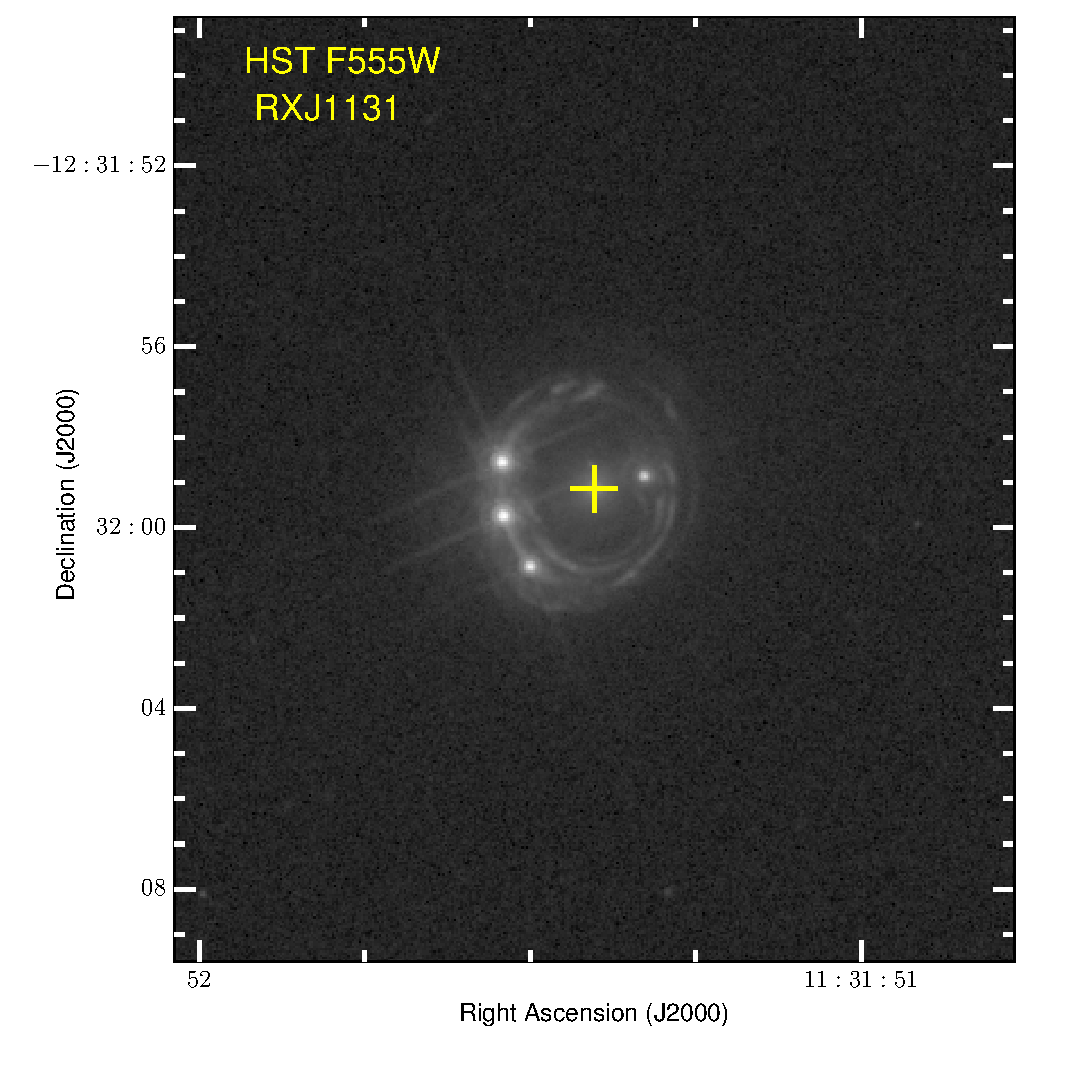
\includegraphics[trim= 10 20 15 0, clip, scale=0.3]{Fig/F555W} % &
%\hspace{-0.5em}
%\includegraphics[trim= 10 0 0 0, clip, scale=0.37]{Fig/Manipulate_figsCROP}
%\vspace{-1em}
%\caption{ \fontsize{10pt}{12pt}\selectfont 
%{
%\textbf{Stellar light distribution in the AGN host galaxy of RXJ 1131-1231 and its reconstructed source plane
%morphology}
%{\em Left:} The rest-frame UV emission (tracing recent star formation) 
%is lensed into an almost complete Einstein ring with diameter $\sim$ 3.8". 
%{\em Right:} Lens modeling of the optical emission identifies complex structure in the host galaxy and
%an optically faint companion (white; \citealt{Claeskens06a}), 
%which we have recently confirmed by modeling \bco emission detected with NOEMA
%(\Fig{combine}; Leung \& Riechers, in prep.). 
%We here propose to study
%the ISM conditions in this AGN-starburst composite system and offers an unparalleled
%view into the early universe, with finer
%detail than otherwise possible with current facilities. 
%}
%\label{fig:HST}}
%\end{figure}

\begin{figure}[!tbhp]
\centering
\floatbox[{\capbeside\thisfloatsetup{capbesideposition={right,center},capbesidewidth=0.425\textwidth}}]{figure}[\FBwidth]
{
\hspace{-0.35em}
\vspace*{-0.55em}
\raggedleft
\caption{ \fontsize{10pt}{12pt}\selectfont 
{
\textbf{Stellar light distribution in the AGN host galaxy of RXJ 1131-1231 and its reconstructed source plane
morphology}
{\em Left:} The rest-frame UV emission (tracing recent star formation) 
is lensed into an almost complete Einstein ring with diameter $\sim$ 3.8". 
{\em Right:} Lens modeling of the optical emission identifies complex structures in the host galaxy and
an optically faint companion (white; \citealt{Claeskens06a}), 
which we have recently confirmed by modeling \bco emission detected with NOEMA
(\Fig{combine}; Leung \& Riechers, in prep.). 
We here propose to study
the ISM conditions in this AGN-starburst composite system and offers an unparalleled
view into the early universe, with finer
detail than otherwise possible with current facilities. 
}
\label{fig:HST}}}
{\hspace{-1em}
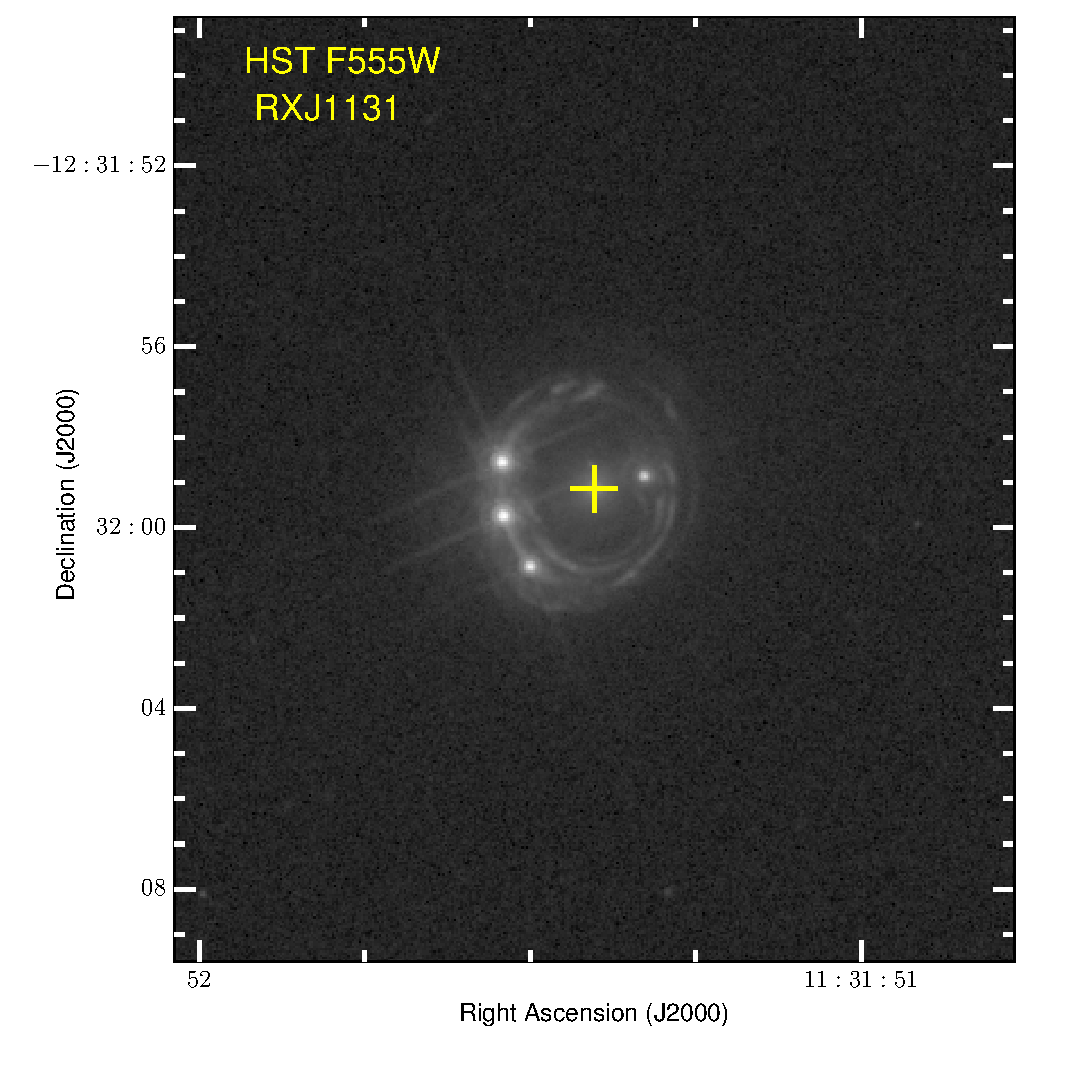
\includegraphics[trim= 10 20 15 0, clip, scale=0.28]{Fig/F555W}
\hspace{-1.5em}
\includegraphics[trim= 10 0 0 0, clip, scale=0.3]{Fig/Manipulate_figsCROP}
\vspace{-1em}
}
\end{figure}
\vspace{-0.8em}
RXJ 1131-1231 is a quadruply imaged AGN with its host galaxy lensed 
into a partial Einstein ring (\Fig{HST}). 
HST observations (rest-frame UV) have revealed distinct emission 
from recent star formation (lensing arcs) and from the AGN (bright knots) in the background galaxy \citep{Sluse03a},
demonstrating the great potential for probing the 
ISM conditions in detail. Lens modeling carried out on optical images shows
that the AGN resides in a star-forming region of size $\sim$0.15" ($\sim$1 kpc)
in its host galaxy, which itself is 1" across ($\sim$7 kpc), and made it possible to identify
seven distinct structures in the source plane (\Fig{HST}). Remarkably, emission originating from 
a spatially offset region ($\sim$2.4 kpc away) from the AGN host galaxy has been identified and found 
to be $\sim$700 pc in size \citep{Brewer08a}, indicating a nearby companion galaxy. 
We have recently confirmed that both galaxies are at the same redshift by detecting their 
\rot[CO]{2}{1} emission and lens-modeling the distribution of the gas in velocity space (\Fig{combine}f), 
verifying that the both are gas-rich (Leung \& Riechers, in prep.). 
Our SED modeling of the dust continuum emission up to 500\,$\mu$m finds $L_{\rm IR}\sim6\times$10$^{12}$\Lsun 
(corrected for lensing). Hence, this target is a gas-rich ULIRG merger at $z$$\sim$0.7 caught in the act. 

%%%%%%%%%%%%%%%%%%%%%%%%%%%%%%%%%%
% \section*{Proposed Observations and Immediate Objectives}
% \vspace{-0.25em}
\noindent {\bf Proposed Observations and Science Goals}
We here propose to map (1): \eco at 0.15" resolution ($\sim$500pc at $z$$\sim$0.7 in the source plane) and 
(2): \dhcn and \dhcop emission at 0.7" resolution (2.5 kpc) and the underlying continuum.
% The science goals at the proposed resolutions are designed to 
The continuum emission traces the optically-thick dust emission, which 
will provide better constraints on the dust temperature(s), dust mass,
and spatial distribution, and thus a tighter constraint on the surface density of the SFR and 
the gas-to-dust ratio. These quantities are key to investigate how the ISM conditions 
vary as galaxies evolve.
In conjunction with the large set of ancillary data from
rest-frame UV to radio wavelength and our new spectral line observations of \bco and \rot[CO]{3}{2}, our
proposed observations will enable a detailed characterization of 
merger/ULIRG in the following aspects.

\underline{\bf Dynamics and kinematics:}
Our recently obtained \bco data shows an asymmetric double-horned line profile (\Fig{combine}a). Given
the observed 1$^{\rm st}$ moment map and the velocity gradient
across the source plane in our model (\Fig{combine}c \& \ref{fig:combine}f), this is indicative of
a kinematically ordered (reminiscent of a rotating disk) galaxy but its emission 
has been lensed differentially. 
Limited by the spatial resolution of this data, it is insufficient to infer the true 
kinematics due to beam smearing.
Furthermore, the unusually high velocity dispersion 
$\gtrsim$400\kms at the central region (\Fig{combine}d) hints at 
perturbations from the central AGN and/or
internal turbulent motion due to interactions with the companion
and/or instability due to the huge gas reservoir.
Thus, higher-resolution imaging, as proposed here, will allow us to
distinguish the major mechanism driving the starburst: merger-driven 
versus gas-rich clumpy disk, since we will also be able to obtain a detailed
dynamical lens modeling of the system.

The \eco observations at 0.15" are complementary to the optical images,
allowing a comparison between the stellar and gas distribution. 
%{\bf The proposed observations will provide the data tracing 
% the warm, excited, dense molecular gas distribution and kinematics, 
% which we will compare against the diffuse component (traced by our already obtained lower-J CO data). 
% OR 
Additionally, since \eco, \dhcn and \dhcop trace the warm, excited, dense molecular gas,
this will allow us to compare against the relatively unperturbed large-scale 
molecular environment and the dynamical mass with our existing lower-$J$ CO data.
% to study the
% gas distribution and kinematics.
Such comparison are key to understand the processes and timescales regulating star-formation 
in ULIRG/merger, and examine how they differ from other galaxy populations.

\underline{\bf Line ratios as AGN/starburst diagnostic:}
By measuring \dhcn/\dhcop in the 
AGN host galaxy, separated from the companion, we will assess its fidelity as a 
AGN/SB diagnostic at higher redshifts than current studies. 
We will as well measure this ratio in the companion and examine the possibility of a 
heavily-obscured AGN at its center. 
Due to the high critical densities of these high-$J$ transitions (\ncrit$\sim$10$^{8}$cm$^{-3}$), 
the \dhcn/CO and \dhcop/CO line ratios are expected to 
be enhanced in AGNs on a global scale, enabling us to carry out a consistency check against the
\dhcn/\dhcop line ratio diagnostic.

The high spin rate of the central black hole in RXJ1131-1231 (over half the speed of light; \citealt{Reis14a})
%(M$_{\rm BH}$$\sim$2$\times$10$^{8}$M$_{\odot}$) 
suggests that the black hole has grown via merger
%[, which provided sufficient accreting materials for
%the observed spin rate,] 
rather than from small episodic accretions (from random directions).
% In contrast if black holes grow through many small accretion episodes, 
% they will accumulate material from random directions, and reduce spin.
In this scenario, the companion and the AGN host galaxy may have already encountered previously.
Therefore, our observations will improve our understanding 
on the formation and evolution of supermassive black holes
and the co-evolution with their host galaxies (and mergers).
More interestingly, we might be witnessing the 
pre/post merging/encounter of two AGN host galaxies if we find evidence of a buried AGN in the companion, 
of which the proposed observations are needed to provide such clues.

\underline{\bf Spectral line energy distributions (SLED) and the SF Law:}
On top of using \dhcn and \hcop as AGN/SB diagnostic, another 
 aspect 
 %for obtaining the proposed line observations 
 is to 
% constrain the ISM conditions by fitting radiative transfer models.
% since these molecular species
% have different excitation criteria. %Therefore, 
%In combination 
combine them with \eco %, \dhcn, and \dhcop line emission
and our existing low-$J$ CO data to perform radiative transfer modeling 
% [with assumptions on their relative abundances] 
to constrain the physical conditions 
(e.g. density and gas kinetic temperature) of the multi-phase molecular gas.
The \dhcn and \dhcop lines are essential as they trace beyond the $J$-transition of the CO SLED turnover
(typically beyond $J$=6\rarr5 in local (U)LIRGs and high-z starbursts; \citealt{Greve14a}).
% and since \eco traces the high kinetic temperature component. 
In addition, since ISM studies of high-z galaxies typically adopt local SLED for comparison \citep[e.g.][]{Bothwell13a}
and/or for asserting assumptions on the conditions of these high-z galaxies.
%[due to the sparsely sampled SLED at high-z \citep{CW13}].
Our observations will thus form a template at z$\sim$0.7 
for these high-z studies.

The ``star-formation law" (%$\Sigma_{\rm SFR}$=$A\Sigma^N_{gas}$ or 
log\LIR=$\alpha$ log\Lp[X]+$\beta$)
is one of the key ingredients % /observational constraints 
for theoretical models as it encodes the physical processes 
of star-formation and its dependence on the ISM 
%(in the slopes and normalizations; 
(e.g. \citealt{Narayanan14a}).
% Observational constraints for the \LIR-\Lp[X] (\Lp of different lines) relations are vital.
However, the \LIR-\Lp[X] at high critical density are currently poorly constrained due to the lack of observations 
and are largely limited to the nearby universe
\citep[\Fig{SF};][]{Greve14a}. Our proposed observations will help delineate 
the slopes at high critical densities and 
explore the linear correlations found 
locally in \Lp[\dhcn]-\LIR and \Lp[\dhcop]-\LIR (\Fig{SF}; Z14) at higher redshifts.
%
\begin{figure*}[!tbph]
\centering
\includegraphics[trim=15 0 5 10, clip, width=0.2\textwidth]{Fig/Zhang}
\includegraphics[trim=5 5 5 10, clip, width=0.2\textwidth]{Fig/Zhang2}
\includegraphics[trim=10 0 0 5, clip, width=0.38\textwidth]{Fig/Greve14Fig2}
\caption{ \fontsize{10pt}{12pt}\selectfont {\textbf{The SF law: log \LIR = $\alpha$ log \Lp[X]+$\beta$.}}
{\em Left \& middle:}
A linear correlation between \LIR-\dhcn and \LIR-\dhcop have been established toward nearby galaxies 
% with \LIR$\sim$10$^9$-10$^{12}$\Lsun 
(Z14), demonstrating the utility of mid-$J$ lines in tracing 
the star-forming dense gas, which will be routinely mapped in high-z galaxies with ALMA.
Our proposed observations will testify the linearity by adding measurements of a ULIRG at z$\sim$0.7, 
% extending the statistics/data to higher redshifts, 
and unveil potential deviations at higher redshift.
{\em Right:} \textbf{Constraints on the SF law 
with line transitions of different \ncrit.}
Most observations are incompatible with current model predictions (gray shaded area),
especially for \dhcn
\citep{Greve14a}.
Our proposed observations will thus reduce the uncertainties on the slopes at high critical densities
and improve our current understanding of galaxy evolution.
\label{fig:SF}}
\end{figure*}

%%%%%%%%%%%%%%%%%%%%%%%%%%%%%%%%%%%
\noindent {\bf Technical overview}
We propose to observe the \eco line at 0.15" resolution
and the \dhcn and \dhcop lines at 0.7", assuming a line 
of 700\kms based on our \bco data
and a source size from our lens model (see details in TJ).
%, which takes into account the asymmetric line emission and spatial extent due to differential lensing. 
We thus expect the source to be resolved over 153 beams 
and 7 beams at 0.15" and 0.7", respectively. 
We compute the target sensitivities for both science goals based on the \bco line flux. 
For \eco, we adopt conservative 
line ratios measured for SMGs \citep[][see TJ for details]{CW13},
and those based on (U)LIRGs for \dhcn (GS04; \citealt{Papadopoulos07a}).
For \dhcop, we adopt the line ratio \dhcn/\dhcop found in ULIRGs 
\citep{Greve09a}. 
We use the most stringent sensitivity estimates 
among \dhcn and \dhcop as our sensitivity goal for science goal $1$. %The latter sets the overall requirement. 
To secure enough S/N for lens modeling, 
we require a minimum of 8$\sigma$ of 0.47 mJy beam\pmOne and 0.07 mJy beam\pmOne
per 150 \kms channel 
%to reconstruct the dynamical structure in the source plane 
for the science goals, respectively. 
We therefore request a \textbf{total time of 7.0 hours}.% to complete our science goals. 

%%%%%%%%%%%%%%%%%%%%%%%%%%%%%%
% closing
\par 
Our proposed observations present an exceptional opportunity to investigate
the physical properties and dynamical structures of 
%different gas phases in 
the ISM in mergers at the cosmic epoch 
where the SFR density is steeply rising \citep{LeFloch05a}, 
connecting high redshift and nearby studies to improve our understanding of galaxy evolution.
%Our proposed observations are vital
%% between the \LIR, SFR$_{\rm IR}$, SFR$_{\rm UV}$, surface densities of SFR, CO, HCN and \hcop,
%to provide constraints on the relation between the ISM and AGN/SB acitvities
%on sub-kpc scales and on the mechanisms driving the vast SFR at earlier epochs, 
%giving rise to the observed stellar-assembly history.
%
This will also % lay the groundwork to 
serve as a benchmark demonstrating the future prospects for ALMA in 
utilizing high-dipole moment molecules as routine tracers to study star-formation 
at high redshifts.

\begin{figure*}[tbph]
\centering
\includegraphics[trim=7 6 5 5, clip, width=0.75\textwidth]{Fig/combine}
\caption{ \fontsize{10pt}{12pt}\selectfont {}
{\em (a):}
The \bco spectrum of RXJ1131-1231 shows a double-horned, highly 
asymmetric line profile, which arises due to differential lensing.
{\em (b):}
Spatial variations traced by \bco as shown by the (red, green, blue) contours corresponding
to the line flux of different velocity channels (red wing, line center, blue wing). 
{\em (c):} 
The observed velocity gradient is suggestive of a kinematically ordered disk at 
the current resolution limit.
{\em (d):} 
Velocity dispersion map of the \bco emitting gas. 
However, limited by the spatial resolution, beam smearing strongly decreases
large-scale velocity gradients and increases observed dispersion.
% RGB spectra
{\em (e): }
Overlay of spectra taken at three locations along the strongest velocity gradient, demonstrating 
differential lensing of the different kinematic components of the galaxy. 
% Lens model
{\em (f): }
Velocity channels of the CO emission toward the gas-rich merger (red contours) overlaid on our best-fit 
lens model for each velocity bin (grayscale). 
The foreground lensing galaxy is represented by a black dot, and 
the beam size is shown in the bottom right corner.
Clearly, there are spatial variations across different kinematic components.
The reconstructed source morphology (magenta ellipses) is suggestive of a kinematically ordered galaxy. 
Given the presence of a companion galaxy within 2.4 kpc and beam smearing effects, high-resolution 
imaging is thus necessary to unambiguously determine the nature that gives rise to the observed velocity gradient
and dynamics, as proposed here.
This will confirm if the system is rotationally supported or highly turbulent 
(tidally disrupted) and allow us to investigate the major mechanisms responsible 
for the starburst in the AGN host galaxy
and investigate whether dominant mode of star formation is GMC-like in a rotating disk or due to fragmentation of
dynamically unstable gas-rich disk. 
{\bf We here aim BLAH}
and provide observational constraints on the star-formation and 
stellar-assembly history at the epoch where the SFR density is steeply 
rising across cosmic times.
\label{fig:combine}}
\end{figure*}
%


\noindent \bf {References}
{\fontsize{10pt}{12pt}\selectfont
	\bibliography{RXJ_ALMAC4}
}

\end{document}
